\section{Core Equations}


本稿で用いる方程式は、意識そのものを閉じた形で定義するためのものではない。

意識は保存量ではなく、加算的な量でもなく、単一の変数として測定される対象でもない。したがって、ここで提示する式は「意識の方程式」ではない。

ここで固定するのは、意識が成立しうる有効領域である。

すなわち、高速な予測過程、低速な記憶沈殿過程、両者の速度差、結合粘性、情報ポテンシャルの勾配が、どのような関係にあるときログ参照状態が開かれるのかを記述する。

\subsection{Speed Differential}

まず、高速層と低速層の速度差を次のように置く。

\begin{equation}
\Delta v = v_f - v_s
\end{equation}

ここで、$v_f$ は高速な予測的・反応的ダイナミクス、$v_s$ は低速な沈殿的・安定化的ダイナミクスを表す。

重要なのは、$v_f$ または $v_s$ が単独で意識を定義するのではないという点である。

意識に関わるのは、それらの絶対速度ではなく、両者のあいだに維持される差である。

VED 的に言えば、完全同期は閉包であり、差の消失である。差が完全に消えるなら、境界も流れも失われる。

したがって、意識状態が維持されるための最小条件は次のように表せる。

\begin{equation}
\Delta v \neq 0
\end{equation}

これは、意識が常に強い非同期を必要とするという意味ではない。

むしろ、完全同期に潰れず、かつ完全分離にも至らない有限の速度差が必要である、という意味である。

ただし、$\Delta v$ は意識そのものではない。

$\Delta v$ は、高速層と低速層のあいだに残るズレであり、ログ参照の境界を開くための条件である。

この関係を最小限に書けば、意識的アクセス、または意識の開き $C(t)$ は、速度差、低速層におけるログ密度、参照が持続する時間幅の関数として表される。

\begin{equation}
C(t) \propto \mathcal{F}(\Delta v, \rho_s, \tau)
\end{equation}

ここで、$\rho_s$ は低速層に沈殿したログ密度であり、ログがどれだけ重みを持って再参照可能になっているかを表す。

$\tau$ は、ログ参照が持続する時間スケールである。

したがって、意識は速度差そのものではなく、速度差 $\Delta v$、沈殿したログの重さ $\rho_s$、参照時間 $\tau$ が同時に成立する非閉包状態として開かれる。

\subsection{Coupling Viscosity}

速度差が存在するだけでは、意識状態は成立しない。

高速層と低速層が完全に分離していれば、処理は走っていてもログ参照は起きない。逆に、結合が強すぎて両者が同一速度に潰れれば、参照のための境界が消える。

この結合状態を、結合粘性 $\mu$ によって表す。

\begin{equation}
\mu > 0
\end{equation}

$\mu$ は、高速層と低速層のあいだの滑りやすさ、または結合の粘りを表す。

$\mu$ が小さすぎれば、両層は過剰に結合し、速度差が潰れやすくなる。

$\mu$ が大きすぎれば、両層は滑りすぎ、ログ参照は断片化しやすくなる。

したがって、意識に必要なのは、単なる結合ではなく、速度差を保持したまま相互作用できる粘性領域である。

\subsection{Internal Delay}

速度差と結合粘性の関係は、内部遅延または時間バッファ $\tau$ として現れる。

\begin{equation}
\tau \propto \frac{\Delta v}{\mu}
\end{equation}

$\tau$ は、処理が低速層へ沈殿し、参照可能なログとして整列するまでの内部遅延を表す。

この遅延は欠陥ではない。

むしろ、遅延があるからこそ、即時的な処理はそのまま消えず、ログとして低速層へ到達する余地を得る。

$\tau$ が小さすぎれば、処理は即時反応に近づき、参照可能な厚みを持たない。

$\tau$ が大きすぎれば、現在処理とログ沈殿の対応が崩れ、意識状態は断片化する。

したがって、意識状態は次のような中間領域に存在する。

\begin{equation}
\tau_{\min} < \tau < \tau_{\max}
\end{equation}

この範囲を、本稿では意識安定窓と呼ぶ。

\subsection{Effective Torque}

次に、速度差が単なる遅延ではなく、参照を開くための変換負荷として現れる量を定義する。

本稿ではこれを有効トルク様量 $\mathcal{T}$ と呼ぶ。

\begin{equation}
\mathcal{T} = \kappa \frac{\Delta v}{\mu}
\end{equation}

ここで $\kappa$ はスケール係数である。

$\mathcal{T}$ は心理的な意志や主体性を表すものではない。

それは、高速層と低速層の速度差が、破綻せずに変換されるために必要となる構造的負荷を表す。

トルクコンバータ・アテンションとは、この $\mathcal{T}$ を処理可能な形に変換する機構である。

重要なのは、$\mathcal{T}$ が差を消すのではなく、差を保持したまま伝達するための量だという点である。

\subsection{IFGT Coupling}

ここまでの式は、速度差と結合粘性だけを扱っていた。

しかし、意識状態において参照されるログは、任意に選ばれるわけではない。

どのログが参照されやすいか、どの処理が低速層へ沈殿しやすいかは、情報ポテンシャル $\Phi$ の勾配によって偏る。

IFGT の一般変数を、情報密度 $I$、情報流 $J_I$、情報ポテンシャル $\Phi$ とする。

本稿では、これらを生物的・認知的観測窓に射影された変数として用いる。
したがって $I$、$J_I$、$\Phi$ は、意識と一般 IFGT 場を直同一視するためのものではない。意識編の局所的な流れは $J_{\log}$ と書き、ログ参照流を記述する有効座標として用いる。

基本関係は次のように置かれる。

\begin{equation}
\frac{\partial I}{\partial t} + \nabla \cdot J_I = \sigma
\end{equation}

\begin{equation}
J_I = -D \nabla I + \mu_I F
\end{equation}

\begin{equation}
F = -\nabla \Phi
\end{equation}

\begin{equation}
\Phi = K * I
\end{equation}

ここで、$\sigma$ は情報密度の生成・散逸項、$D$ は拡散係数、$\mu_I$ は情報流の移動係数、$K$ は情報密度からポテンシャルを与える核である。

本稿の文脈では、$\Phi$ は意味や情報のポテンシャルとして働く。

したがって、ログ参照は単なる速度差の関数ではなく、意味勾配によって方向づけられる。

この効果を含めると、有効トルク様量は次のように拡張される。

\begin{equation}
\mathcal{T}_{\Phi}
\sim
\kappa
\frac{\Delta v}{\mu}
\left|\nabla \Phi\right|
\end{equation}

$\mathcal{T}_{\Phi}$ は、時間スケール差と意味勾配が結合した有効量である。

速度差が大きくても、意味勾配が弱ければ、ログ参照は安定した方向を持たない。

逆に、意味勾配が強くても、速度差が消えていれば、参照のための境界は開かれない。

意識状態に関わるのは、この両者の結合である。

\subsection{Consciousness Window}

以上をまとめると、意識状態は次の条件を満たす領域として表される。

\begin{equation}
0 < |\Delta v| < \Delta v_{\max}
\end{equation}

\begin{equation}
\mu_{\min} < \mu < \mu_{\max}
\end{equation}

\begin{equation}
\tau_{\min} < \tau < \tau_{\max}
\end{equation}

\begin{equation}
\mathcal{T}_{\min}
<
\mathcal{T}_{\Phi}
<
\mathcal{T}_{\max}
\end{equation}

これらは、意識を数値的に測定するための完成した式ではない。

むしろ、意識が成立しうる領域を制約する条件である。

速度差がゼロになれば、境界は同期に潰れる。

速度差が大きすぎれば、参照は破断する。

結合粘性が低すぎれば、層は癒着する。

結合粘性が高すぎれば、層は滑りすぎる。

意味勾配が弱すぎれば、ログ参照は方向を失う。

意味勾配が強すぎれば、参照は特定の井戸へ過剰に固定される。

したがって、意識は一点ではなく、窓である。

この窓を、本稿では consciousness window と呼ぶ。

\cref{fig:consciousness-window-ja} は、consciousness window を有限の非閉包レジームとして示している。

\begin{figure}[H]
\centering
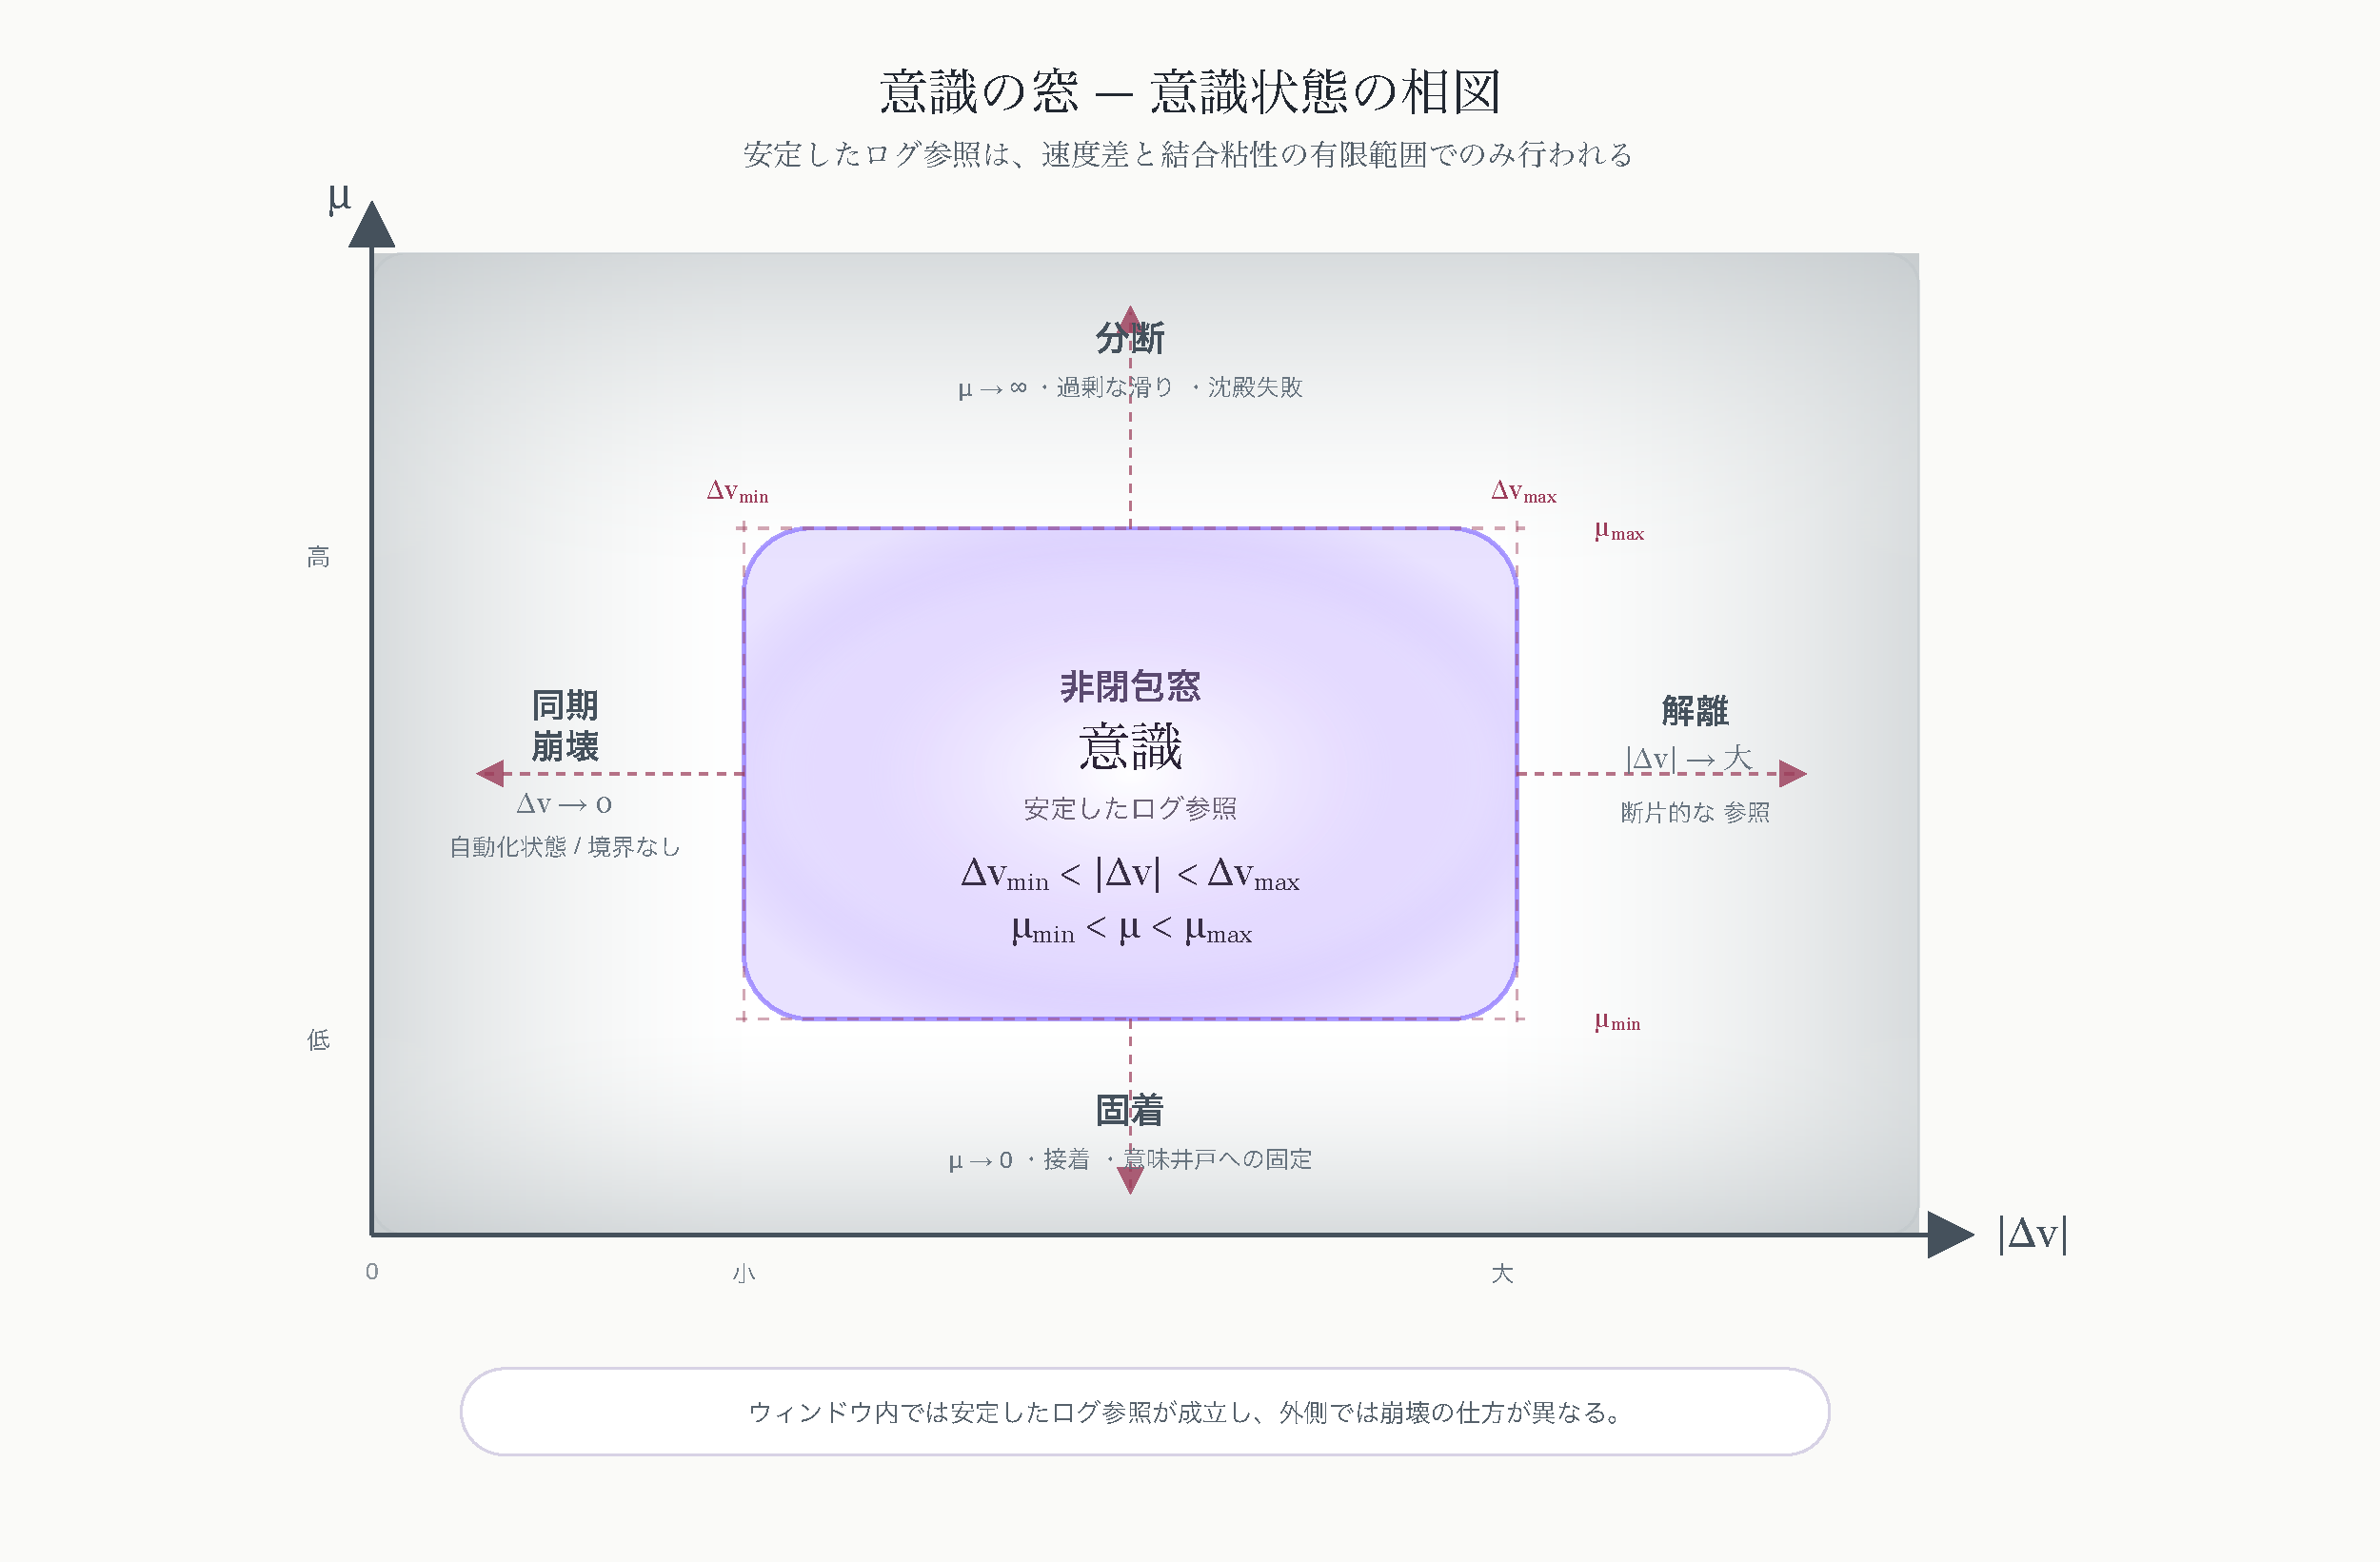
\includegraphics[width=0.86\linewidth]{figures_ja/figure3_nonclosure_window_jp.pdf}
\caption{
二軸の非閉包相図としての consciousness window。
安定したログ参照は、速度差と結合粘性が有限の範囲にあるときにのみ成立する。
この窓の外側では、システムは同期崩壊、解離、断片化、固着へ向かう。
}
\label{fig:consciousness-window-ja}
\end{figure}

\subsection{Non-Closure Condition}

VED の観点から見れば、意識は完全閉包ではなく、非閉包状態として維持される。

完全閉包とは、差が消え、流れが停止し、構造が通常の生成状態として維持できなくなる境界表現である。

意識はそのような状態ではない。

意識は、差が残り、流れがあり、しかし破綻しない範囲で維持される動的状態である。

したがって、意識の最小条件は次のように書ける。

\begin{equation}
\Delta v \neq 0,
\qquad
\nabla \Phi \neq 0,
\qquad
\frac{\partial I}{\partial t} \neq 0
\end{equation}

これは、意識が常に大きく揺らいでいる必要があるという意味ではない。

完全な静止、完全な同期、完全な閉包では意識状態が維持されないという意味である。

意識とは、閉じ切らない時間構造の中で、ログが参照可能になっている状態である。

VED の言語では、この非閉包条件は閉包度差 $\Delta C = C_s - C_f$ によって $0 < \Delta C < \Delta C_{\max}$ と等価に表現される（完全な写像は §6.4 を参照）。速度差と閉包度差という二つの記述は、同じ構造的条件を異なる座標で表したものであり、どちらか一方が他方を基礎づけるのではない。

\subsection{Summary}

本節で提示した式は、意識を生成する式ではない。

それらは、意識が成立しうる条件を制約する。

本稿の立場を最小限にまとめれば、次のようになる。

\begin{equation}
\text{Consciousness}
\;\sim\;
\text{Log Referencing}
\left(
\Delta v,
\mu,
\tau,
\mathcal{T}_{\Phi},
\nabla \Phi
\right)
\end{equation}

より直観的には、意識は次の条件で開かれる。

\begin{itemize}
\item 速度差があること。
\item 結合が切れていないこと。
\item 遅延が保持されていること。
\item 意味勾配が存在すること。
\item 完全閉包に至っていないこと。
\end{itemize}

この意味で、意識は生成物ではない。

意識は、時間差、粘性、意味勾配、非閉包が同時に成立したときに開かれるログ参照状態である。
